\documentclass{article}
\usepackage[margin=0.6in]{geometry}
\usepackage{amsmath}
\usepackage{amssymb}
\usepackage{bookmark}
\usepackage{graphicx}
\usepackage{float}

\newcommand{\vct}[1]{\mathbf{#1}}
\newcommand{\argmax}{\mathop{\mathrm{argmax}}}
\newcommand{\argmin}{\mathop{\mathrm{argmin}}}

\title{Solutions to the Assignment - 5 : CS5560 - \\
Probabilistic Models in Machine Learning}
\author{Vishwak Srinivasan\\
\texttt{CS15BTECH11043}}
\date{}

\begin{document}
\maketitle

\section*{Exercises from ML: A Probabilistic Perspective}
\subsection*{Exercise 4.19}
\begin{flushleft}
\end{flushleft}

\subsection*{Exercise 4.21}
\subsubsection*{Part a}
\begin{flushleft}
If \(p(x | \mu_{1}, \sigma_{1}) \geq p(x | \mu_{2}, \sigma_{2})\), then \(-2\log p(x | \mu_{1}, \sigma_{1}) \leq -2\log p(x | \mu_{2}, \sigma_{2})\). This means that:
\begin{equation}
\label{r1-eqn}
\frac{(x - \mu_{1})^{2}}{\sigma_{1}^{2}} + \log \sigma_{1}^{2} \leq \frac{(x - \mu_{2})^{2}}{\sigma_{2}^{2}} + \log \sigma_{2}^{2} \Rightarrow x^2 - \frac{(x - 1)^{2}}{10^{6}} - \log (10^{6}) \leq 0 \Rightarrow x^{2}\left(1 - \frac{1}{10^{6}}\right) + x\frac{2}{10^{6}} - \left(\frac{1}{10^{6}} + \log 10^{6}\right) \leq 0
\end{equation}

A graphical sketch is shown below:
\(\newline\)
\begin{minipage}{0.475\linewidth}
\begin{figure}[H]
\centering
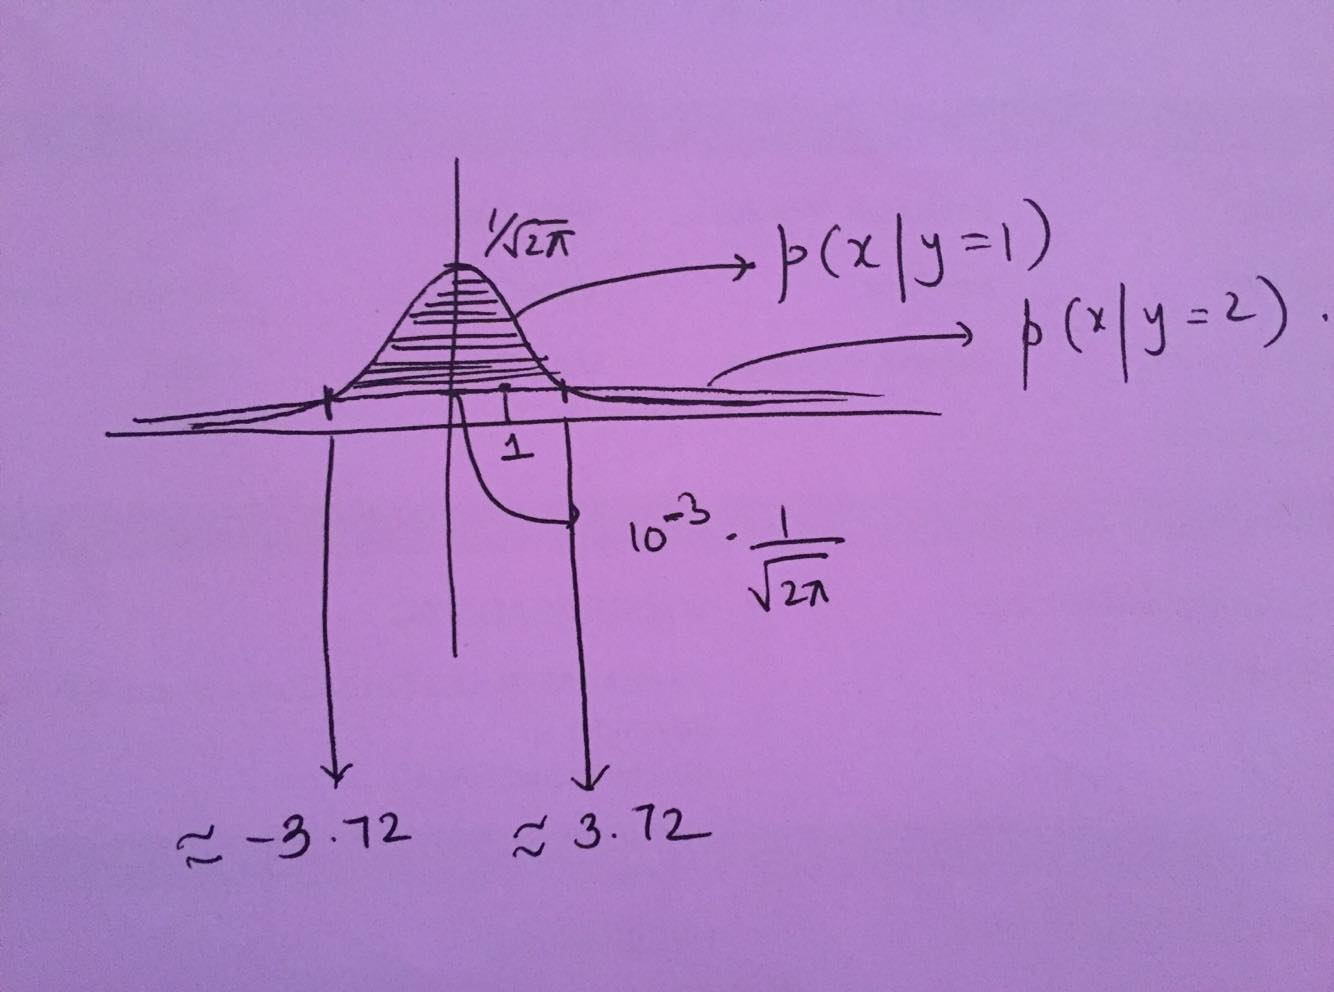
\includegraphics[width=0.6\textwidth]{./images/4_21_a_sketch.jpg}
\end{figure}
\end{minipage}
\hfill
\begin{minipage}{0.475\linewidth}
The domain of the shaded region corresponds to the set \(R_{1}\). The end-points of this domain can be found by solving the equality case in \ref{r1-eqn}. Denote \(C_{1} = 1 - \frac{1}{10^{6}}\), \(C_{2} = \frac{2}{10^{6}}\) and \(C_{3} = -\left(\frac{1}{10^{6}} + \log 10^{6}\right)\).
\begin{multline}
C_{1}x^2 + C_{2}x + C_{3} = 0 \Rightarrow x = \frac{-C_2 \pm \sqrt{C_{2}^{2} - 4C_{1}C_{3}}}{2C_{1}}\\= \frac{-1 \pm 10^{3}\sqrt{10^{6}\log 10^{6} + 1 - \log 10^{6}}}{(10^{6} - 1)}\\\Rightarrow x \approx \pm 3.7169
\end{multline}
\end{minipage}
\end{flushleft}

\subsubsection*{Part b}
\begin{flushleft}
Note that if \(\sigma_{1}^{2} = \sigma_{2}^{2}\), then the first equality in \ref{r1-eqn} would become:
\begin{equation}
(x - \mu_{1})^{2} \leq (x - \mu_{2})^{2} \Rightarrow 2(\mu_{2} - \mu_{1})x \leq \mu_{2}^{2} - \mu_{1}^{2} \Rightarrow x \leq \frac{\mu_{2} + \mu_{1}}{2} = \frac{1}{2}
\end{equation}

\begin{minipage}{0.475\linewidth}
\begin{figure}[H]
\centering
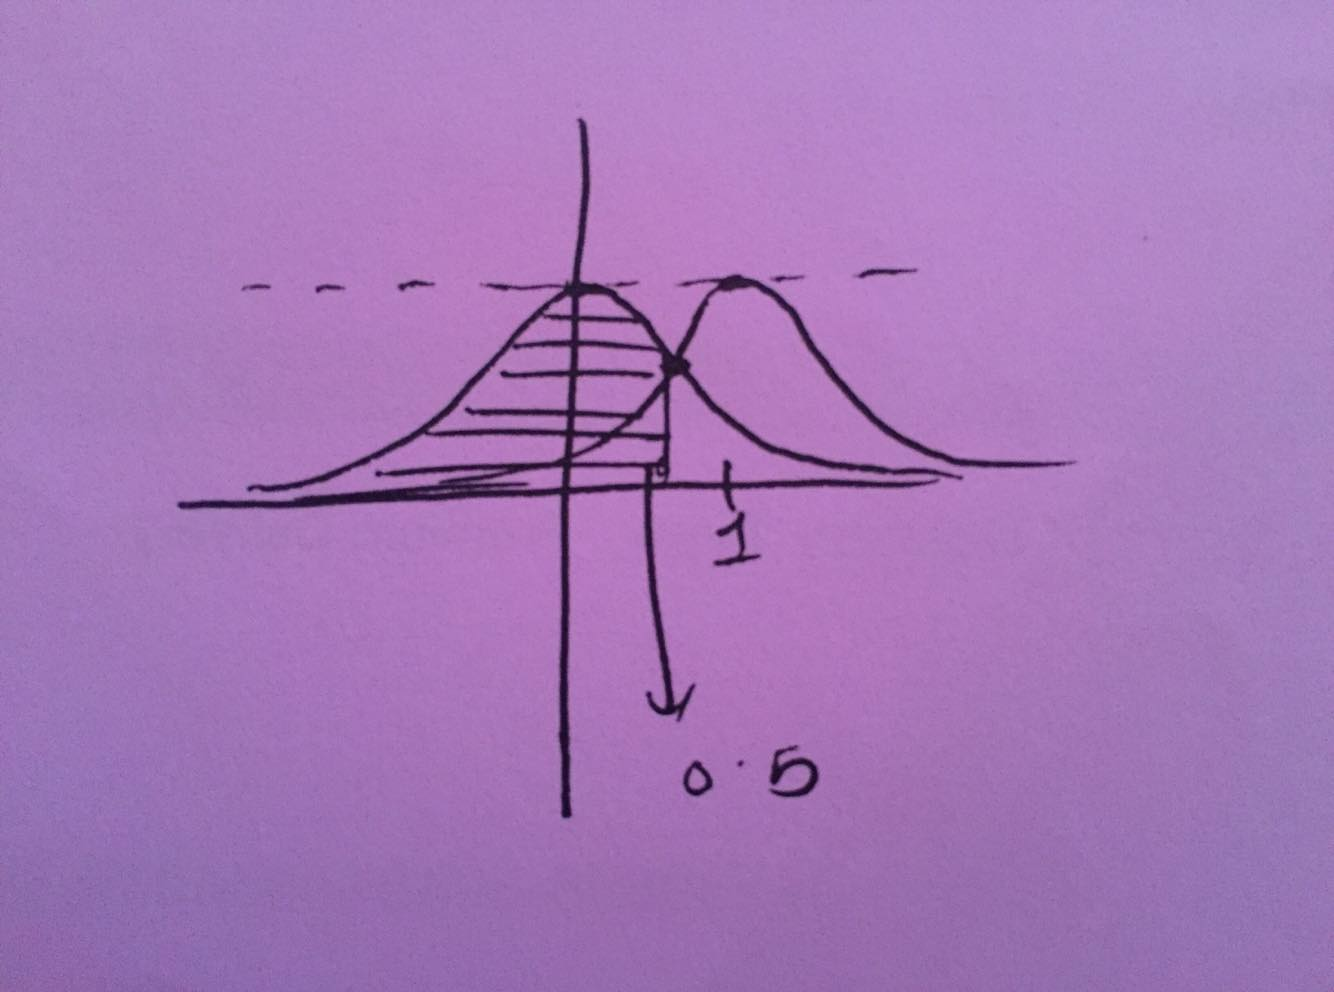
\includegraphics[width=0.6\textwidth]{./images/4_21_b_sketch.jpg}
\end{figure}
\end{minipage}
\hfill
\begin{minipage}{0.475\linewidth}
\(R_{1}\) is the left partition of the real line from \(\frac{1}{2}\).
\end{minipage}
\end{flushleft}

\subsection*{Exercise 4.22}
\begin{flushleft}
Recall that the predictor is given by \(\hat{g}(\vct{x}) = \argmax_{y \in \mathcal{Y}} p(Y | \vct{x} = y)\). Now from the facts in the question:
\begin{equation}
p(y | \vct{x}) \propto p(\vct{x} | y) p(y) \propto p(\vct{x} | y)
\end{equation}

The last proportionality excludes \(p(y)\) due to the fact that the \(P(Y = 1) = P(Y = 2) = P(Y = 3) = \frac{1}{3}\). Now the prediction equation can be re-written as:
\begin{equation}
\hat{g}(\vct{x}) = \argmax_{y \in \{1, 2, 3\}} p(\vct{x} | Y = y) = \argmax_{y \in \{1, 2, 3\}} \log p(\vct{x} | Y = y) = \argmin_{y \in \{1, 2, 3\}} -2\log p(\vct{x} | Y = y) - \log 2\pi
\end{equation}

Some equations to consider:
\begin{gather}
-2\log p(\vct{x} | Y = i) - \log 2\pi= (\vct{x} -\vct{\mu}_{1})^{T}\Sigma^{-1}_{1}(\vct{x} -\vct{\mu}_{1}) + 2\log |\Sigma_{i}|
\end{gather}

\begin{center}
\begin{tabular}{|c|c|c|}
\hline
\(i\) & \(\Sigma_{i}^{-1}\) & \(|\Sigma_{i}|\) \\
\hline
\(1\) & \(\begin{bmatrix} \frac{1}{0.7} & 0 \\ 0 & \frac{1}{0.7} \end{bmatrix}\) & \(0.49\) \\
\hline
\(2\) & \(\begin{bmatrix} \frac{4}{3} & -\frac{1}{3} \\ -\frac{1}{3} & \frac{4}{3} \end{bmatrix}\) & \(0.6\) \\
\hline
\(3\) & \(\begin{bmatrix} \frac{4}{3} & -\frac{1}{3} \\ -\frac{1}{3} & \frac{4}{3} \end{bmatrix}\) & \(0.6\) \\
\hline
\end{tabular}
\end{center}

\subsubsection*{Part a}
\begin{equation}
\hat{g}([-0.5, 0.5]) = \argmin_{y \in \{1, 2, 3\}} \{1.69, 4.03, 2.03\} = 1
\end{equation}

\subsubsection*{Part b}
\begin{equation}
\hat{g}([0.5, 0.5]) = \argmin_{y \in \{1, 2, 3\}} \{1.69, 1.7, 5.03\} = 1
\end{equation}
\end{flushleft}

\section*{Starred Problems}
\subsection*{Problem 2: 8.6 from ML: A Probabilistic Perspective}
\subsubsection*{Part a}
\begin{flushleft}
First we prove that \(f(\vct{w}) = -\log \sigma(y \vct{x}^{T} \vct{w})\) is convex. Now:
\begin{gather}
\frac{df}{dw_{i}} = -\frac{1}{\sigma(y \vct{x}^{T}\vct{w})} \sigma(y \vct{x}^{T}\vct{w}) (1 - \sigma(y \vct{x}^{T}\vct{w})) yx_{i} = (\sigma(y \vct{x}^{T}\vct{w}) - 1) yx_{i}\\
\frac{d^{2}f}{dw_{i}dw_{j}} = yx_{i}\sigma(y \vct{x}^{T}\vct{w})(1 - \sigma(y \vct{x}^{T}\vct{w}))yx_{j}
\end{gather}

Consider \(\vct{z}\) such that \(\vct{z} \neq 0\). Now we know that the matrix formed with the \((ij)^{th}\) entry as \(\frac{d^{2}f}{dw_{i}dw_{j}}\) is the Hessian (denoted by \(\vct{H}\)). To prove that this function is convex, we have to show that \(\vct{z}^{T}\vct{H}\vct{z} \geq 0\) or \(\displaystyle\sum_{i, j = 1} z_{i}z_{j}H_{ij} \geq 0\). We will use the second approach.
\begin{multline}
\sum_{i}\sum_{j} z_{i}z_{j}y^{2}x_{i}x_{j}\sigma(y \vct{x}^{T}\vct{w})(1 - \sigma(y \vct{x}^{T}\vct{w})) = y^{2}\sigma(y \vct{x}^{T}\vct{w})(1 - \sigma(y \vct{x}^{T}\vct{w}))\left(\sum_{i}z_{i}x_{i}\right)\left(\sum_{j}z_{j}x_{j}\right)\\= \sigma(y \vct{x}^{T}\vct{w})(1 - \sigma(y \vct{x}^{T}\vct{w})) \left(\sum_{i} z_{i}x_{i}\right)^{2} \geq 0
\end{multline}

The final step is due to:
\begin{enumerate}
\item \(y^{2} = 1\) for \(y = \{+1, -1\}\)
\item \(\sigma(y \vct{x}^{T}\vct{w}) \in (0, 1) \Rightarrow 1 - \sigma(y \vct{x}^{T}\vct{w}) \in (0, 1) \Rightarrow \sigma(y \vct{x}^{T}\vct{w})(1 - \sigma(y \vct{x}^{T}\vct{w})) > 0\)
\item \(\displaystyle\sum_{i}\sum_{j} a_{i}a_{j} = \sum_{i}a_{i}\sum_{j}a_{j} = \left(\sum_{i}a_{i}\right)\left(\sum_{i}a_{i}\right) = \left(\sum_{i}a_{i}\right)^{2} \geq 0\)
\end{enumerate}

Next the sum of two convex functions are convex. Define \(h(x) = f(x) + g(x)\) where \(f\) and \(g\) are convex. Using Jensen's inequality, for \(\lambda \in [0, 1]\):
\begin{multline}
h(\lambda x_{1} + (1 - \lambda)x_{2}) = f(\lambda x_{1} + (1 - \lambda)x_{2}) + g(\lambda x_{1} + (1 - \lambda)x_{2})\\\leq \lambda f(x_{1}) + (1 - \lambda)f(x_{2}) + g(x_{1}) + (1 - \lambda)g(x_{2})\\= \lambda(f(x_{1}) + g(x_{1})) + (1 - \lambda)(f(x_{2}) + g(x_{2}))=\lambda h(x_{1}) + (1 - \lambda)h(x_{2})
\end{multline}

This can be generalized for as many functions as we want via induction, which means that \(\displaystyle\sum_{i \in \mathcal{D}} -\log \sigma(y_{i}\vct{x}_{i}^{T}\vct{w})\) is convex as well. Scaling by a positive constant doesn't affect convexity, hence \(\displaystyle\frac{1}{|\mathcal{D}|}\sum_{i \in \mathcal{D}} -\log \sigma(y_{i}\vct{x}_{i}^{T}\vct{w})\) is convex as well. Trivially, for \(\lambda > 0\), \(\lambda ||\vct{w}||_{2}^{2}\) is convex, meaning that \(J(\vct{w})\) is convex. Therefore, \(J(\vct{w})\) cannot have multiple optimal solutions. The statement is \textbf{false}.
\end{flushleft}

\subsubsection*{Part b}
L2 regularization can be perceived as optimizing over a circle (in 2D). The critical points attained at the boundary are not sparse, unlike L1 regularization which can be perceived as optimizing over a diamond figure (in 2D), where the points of at which low norm is achieved are the corners of the diamond, effectively nullifying some of the dimensions. The statement is \textbf{false}

\subsubsection*{Part c}
\textbf{True}, as explained in class.

\subsubsection*{Part d}
Increasing the \(\lambda\) parameter, will cause the weights to approach \(0\) more, since the problem is biased towards giving solutions with low norm. This could cause the other component of \(J(\vct{w})\) which is \(-\ell(\vct{w}, \mathcal{D}_{\text{train}})\) to increase. This would hence cause \(\ell(\vct{w}, \mathcal{D}_{\text{train}})\) to decrease. The statement is \textbf{false}.

\subsubsection*{Part e}
Increasing the \(\lambda\) parameter, will cause low-norm (biased) solutions. However, it is not exactly clear if this will be good for the testing set, even though it is clear it is not good for the training set, and hence may not always be the case. The statement is \textbf{false}.

\subsection*{Problem 2: 8.7 from ML: A Probabilistic Perspective}
\subsubsection*{Part a}
\begin{minipage}{0.475\linewidth}
\begin{figure}[H]
\centering
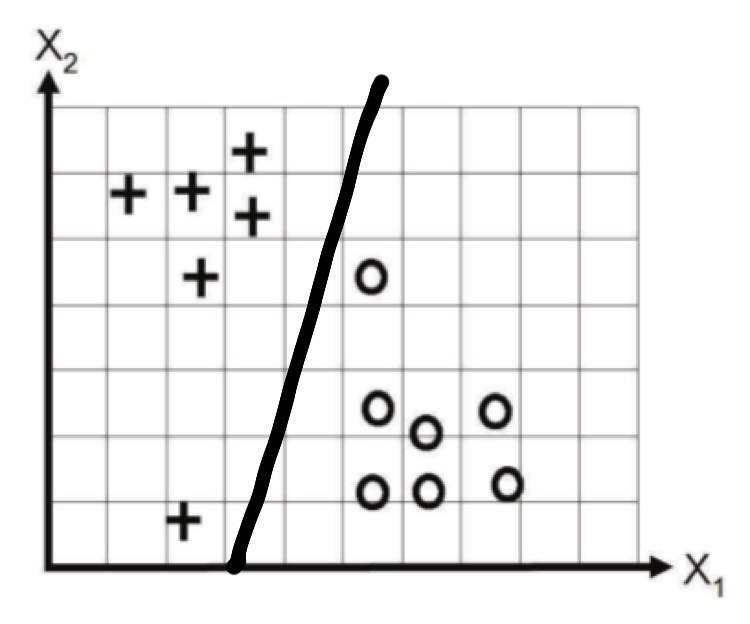
\includegraphics[width=0.6\textwidth]{./images/8_7_a.jpg}
\end{figure}
\end{minipage}
\hfill
\begin{minipage}{0.475\linewidth}
The boundary is basically the line \(w_{0} + w_{1}x_{1} + w_{2}x_{2} = 0\). Now, scaling the weights will not affect this boundary, meaning that the drawn line is not the unique solution for the problem. There are no classification errors made on the training dataset.
\end{minipage}

\subsubsection*{Part b}
\begin{minipage}{0.475\linewidth}
\begin{figure}[H]
\centering
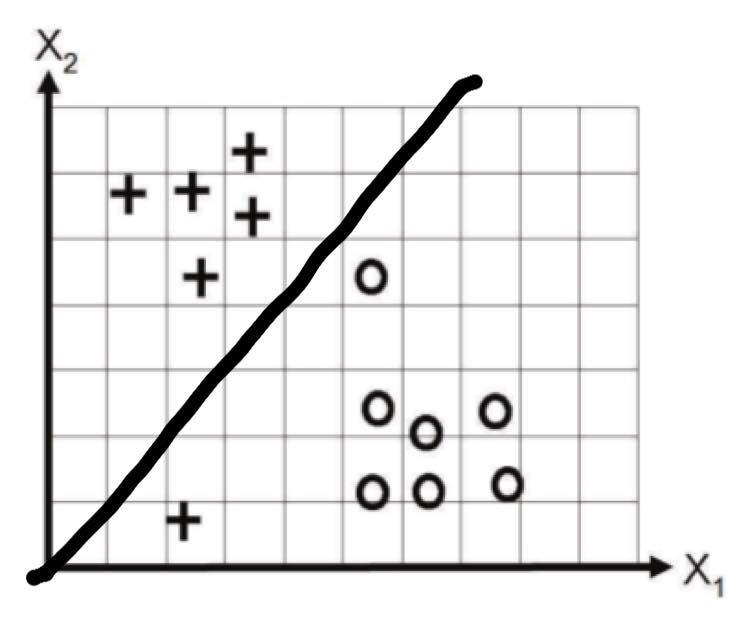
\includegraphics[width=0.6\textwidth]{./images/8_7_b.jpg}
\end{figure}
\end{minipage}
\hfill
\begin{minipage}{0.475\linewidth}
The boundary is basically the line \(w_{0} + w_{1}x_{1} + w_{2}x_{2} = 0\). Since the intercept term is regularized down to 0, the boundary would be a line very close / passing through the origin. There will be one classification error.
\end{minipage}

\subsubsection*{Part c}

\subsubsection*{Part c}

\subsubsection*{Part d}
\end{document}
